\section{Research method}\label{sec:research_methods}

\subsection{GRATiS Design}
The specific method used to achieve the design goal is to use GROOVE as a replacement of the STS in ATM. Figure~\ref{fig:tooling} shows this graphically. The Rule Applier component now communicates with the Interface, which fulfills the role of STS Engine. The communication runs through interfaces on both tools, such that other tools are also able to communicate with the GROOVE component. The possible rule transitions are translated by the Interfaces to possible transitions for the Test Manager. The chosen transitions are translated back to rule transitions by the Interfaces.

\begin{figure}[h]
  \begin{center}
    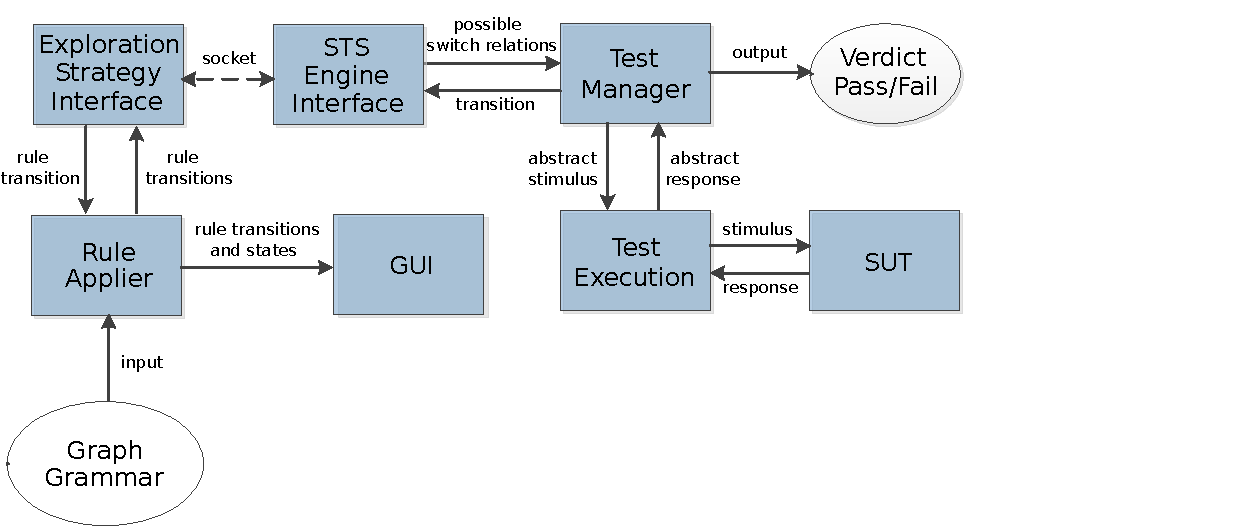
\includegraphics[width=\textwidth]{tooling.pdf}
  \end{center}
  \caption{The GRATiS design: replacing the STS with GROOVE}
  \label{fig:tooling}
\end{figure}

\subsubsection{Problems}\label{sec:problems}
The boardgame example revealed some problems, listed below, for the GRATiS design. These need to be tackled during the design phase of the project. 
\begin{itemize}
  \item Modelling data types such as integers and strings in GROOVE is problematic; the range of possible values has to be given explicitly and cannot be infinite. For example, it would be impossible to extend the die of the boardgame example such that it can throw any integer; each value of an integer would have to be defined separately.
  \item In order to efficiently define transitions with a rule system, sometimes one transition is represented by multiple transitions. In the case of the boardgame example, the \textbf{Player} node moves to the next \textbf{Location} node a number of times equal to the number thrown with the die, as shown in Figure~\ref{fig:statespace_groove1}. A concrete response from the SUT, where the player moves to any location but the next, would need to be translated to a number of 'move' transitions as the abstract response. Otherwise the Test Manager observes this action as erroneous behavior. This translation introduces coupling between the Test Execution component and the specific model. The modularity of these components is therefore lost. %Either the multiple move transitions need to be translated into one abstract label representing the complete movement or the concrete label needs
\end{itemize}

\subsubsection{Coverage}
ATM annotates the locations it has seen and the switch relations it has chosen in the STS. These annotations are needed to calculate the coverage statistics. GRATiS must therefore be able to determine the location of a graph state, by abstracting from the concrete data values in the graph state.

Also, as mentioned in section~\ref{sec:sts_coverage}, the calculation of data coverage for a test run will be implemented in GRATiS.

\subsubsection{Initial design step: GRATiS-Min}
Before the problems in \ref{sec:problems} are tackled and the design of GRATiS implemented, an initial design that minimally achieves the design goal is implemented. This initial design, named GRATiS-Min performs the following steps:
\begin{enumerate}
  \item generate the GTiS based on the GTS using GROOVE
  \item transform the GTiS to a basic STS
  \item send the STS to ATM
  \item perform the automatic test generation on the STS
\end{enumerate}

There are a number of advantages to GRATiS-Min:
\begin{itemize}
  \item It allows automatic test generation on models which GROOVE is able to fully explore. This has been done on some interesting systems, as described in section~\ref{sec:descriptiongroove}.
  \item It is easy to implement.
  \item It already implements some features of GRATiS, such as the communication between GROOVE and ATM, which makes GRATiS easier to build.
\end{itemize}
And also some disadvantages:
\begin{itemize}
  \item It cannot provide test results on systems with too many states and transitions (for example, due to data values such as integers)
  \item The Test Manager component of ATM cannot use the data values for its test selection strategy, as all values are spread across multiple switch relations. Also, the calculation of location and switch relation coverage statistics on the basic STS will actually reveal the state and transition coverage.
\end{itemize}
The last disadvantage can be solved by providing a better transformation of an LTS to an STS. Constructing such a transformation is a sub-goal of the main design goal, as it improves GRATiS-Min. Therefore, this will be part of the research project.

\subsection{Validation}\label{sec:research_methods_validation}
There are two steps in the validation:
\begin{enumerate}
  \item The boardgame example is tested. A SUT is made for this game and ATM is used to test this game. Then, GRATiS is used to test the boardgame. The results should reveal no errors, fail verdicts or other differences in the output of both tools. An intentional error is then made in the SUT and the process is repeated. Still no errors or differences are expected, but both tools should find the error and give a fail verdict.
  \item Next, the assessment of the strengths and weaknesses of GRATiS is done by applying both tools to several case studies and comparing the results. The case studies are set out first and then the criteria for the comparison are given.
\end{enumerate}

\subsubsection{Case studies}
Three case studies are planned. They are all real-life systems Axini has worked on:
\begin{itemize}
  \item a self-scan register
  \item a navigation system
  \item a health-care system
\end{itemize}  

The self-scan register is a machine that automates the purchase of products at a supermarket. A customer can put his products on a conveyer belt and the system automatically calculates the price of the products. Then the customer pays and gets a receipt. The navigation system is a GPS device with a route planner. It allows a user to enter a destination and the system plans the correct route accordingly from the location of the user. The health-care system is a medical device.

A GTS and an STS will be created for each system. GRATiS and ATM are used for the automatic test generation on these models respectively. Both the model and the test process will then be compared as part of the validation. The next two sections give the criteria for this comparison.

\subsubsection{Objective criteria}
As mentioned in section~\ref{sec:questions}, the criteria for the comparison of ATM and GRATiS are split in two parts. The objective criteria that can be compared are:
\begin{enumerate}
  \item The verdicts: same test cases should give same verdicts. When a verdict is different for the same test case in GRATiS and ATM, this might indicate an error.
  \item The number of bugs found: one tool could generate smarter test-cases and find more bugs.
  \item The coverage: generating smarter test-cases can also lead to a higher coverage.
  \item The test cases generated per second: benchmarks will be done on how fast the tools generate test-cases.
  \item The size of the statespace: benchmarks will be done on how much space the tools use.
\end{enumerate}

\subsubsection{Subjective criteria}
Subjective criteria, such as the maintainability and extendibility of a model, are related to the usability of GTSs versus alternative formalisms, such as STSs. Evaluaiting such criteria requires an extensive experiment with a statistical significant set of human actors. It is out of the scope of this project to perform such an experiment in order to compare two modelling formalisms. In section~\ref{sec:introduction} a motivation is given for the use of GTSs in model-based testing. The qualities of GTSs described there cover the usability of the GTSs.

% the participants are asked to work on one of the case studies. This work entails either:
%\begin{enumerate}
%  \item Extending the model with a new feature
%  \item Finding a bug/error in the SUT/model
%\end{enumerate}
%The following results are then noted and compared:
%\begin{enumerate}
%  \item The time spent on the assignment
%  \item The correctness of the result
%  \item The feelings the participants had with the assignment (how difficult, how much fun, etc.)
%\end{enumerate}

%The results will give insight in the understandibility, maintainability and extendibility of both modelling processes. The results are compiled and presented in the final thesis.
